\documentclass{article}
\usepackage{latexsym}
\usepackage{amsmath}
\usepackage{amssymb}
\usepackage{amsthm}
\usepackage{graphicx}

\newtheorem{theorem}{Theorem}[section]
\begin{document}
\title{Eisenstein Triples: Connecting geometry and number theory}
\author{Dave Neary}

\maketitle

\section{A number theory problem}

We start with a number theory puzzle: Can you find positive integer triples $(a,b,c)$ such that:
\[ \frac{1}{a+c} + \frac{1}{b+c} = \frac{3}{a+b+c} \]

To get started with our exploration, let's clear denominators by multiplying across by
$(a+c)(b+c)(a+b+c)$ to get:
\begin{equation*}
\begin{split}
(b+c)(a+b+c) + (a+c)(a+b+c) & = 3(a+c)(b+c) \\
a^2 + b^2 + 2c^2 + 2ab + 3bc + 3ac & = 3ab + 3ac + 3bc + 3c^2 \\
a^2 - ab + b^2 &= c^2
\end{split}
\end{equation*}

Our goal will be to find positive integer solutions to this equation.

\section{A geometric aside}

This equation may look familiar to anyone who has come across the cosine rule in geometry.
For the sides of a triangle $(a,b,c)$ with opposite angles $(A,B,C)$:

\[ c^2 = a^2 + b^2 -2ab\cos(C) \]

with similar equations for $a^2, b^2$.

Rewriting the equation above in this form, we can see that the problem is equivalent to finding
triangles with integer sides $(a,b,c)$ such that $\cos(C) = \frac{1}{2}$ - that is,
$C = \frac{\pi}{3}$. In other words, our challenge is to find triangles with one angle measuring
$60^{\circ}$ which have integer side lengths.

This is a well known problem that has been explored by many number theorists in the past, and
triples of this form are known as Eisenstein triples, named after the mathematician Eisenstein.

By considering the problem as one of triangles with a certain constraint, perhaps we can approach
this problem the way we would approach finding Pythagorean triples.

\section{Factoring sums of squares}

One way to generate Pythagorean triples is to factor $a^2+b^2$ over the Gaussian integers - that is,
the subset of the complex numbers $a+ib$ with $a,b\in \mathbb{Z}$. In the Gaussian integers, we can 
rewrite $ a^2 + b^2 = a^2 - b^2i^2$ as a difference of two squares - yielding a factorization:
\[ c^2 = a^2 + b^2 = (a+ib)(a-ib) \]

How does this help? Well, if we take an arbitrary Gaussian integer $z = a+ib$, the length of $z$ is
$|z| = \sqrt{a^2+b^2}$ - so if we take the length of $z^2$, we are guaranteed to get an integer
length, since $|z|^2 = |z^2|$. We will have:
\begin{equation*}
	\begin{split} 
		z^2 &= (a+ib)^2 \\
		& = a^2-b^2 + i(2ab) \\
		|z^2| &= \sqrt{(a^2-b^2)^2 + (2ab)^2 }\\
		|z|^2 &= a^2 + b^2 \\
		|z^2| &= |z|^2 \\
		\Rightarrow (a^2-b^2)^2 + (2ab)^2 &= (a^2 + b^2)^2
	\end{split}
\end{equation*}

So if we take \textbf{any} positive integers $(a,b)$, we can generate a Pythagorean triple 
$(a^2-b^2, 2ab, a^2+b^2)$ from them.

Can we use a similar approach with our puzzle? Indeed we can!

\section{Factoring the quadratic in $\mathbb{C}$}

We can factor $a^2 - ab + b^2$ in complex numbers too by setting it equal to zero and using 
the quadratic formula:
\begin{equation*}
	\begin{split} 
		a^2 - ab + b^2 &= 0 \\
		a &= \frac{1}{2}\left(b \pm \sqrt{b^2-4b^2}\right) \\
		&= \frac{b}{2}\left(1 \pm \sqrt{3}i\right)
	\end{split}
\end{equation*}

The factorization is:
\[ a^2 - ab + b^2 = 
\left(a + \frac{b}{2}\left(-1 - \sqrt{3}i\right) \right)
\left(a + \frac{b}{2}\left(-1 + \sqrt{3}i\right) \right) \]

If you have done any complex analysis these roots might look familiar to you. Given 
$z = \frac{1}{2}(-1+\sqrt{3}i)$ then:
\begin{equation*}
        \begin{split} 
		z^2 & = \frac{1}{4}(-1+\sqrt{3}i)^2 \\
		& = \frac{1}{4}(1 - 2\sqrt{3}i - 3) \\
		& = \frac{1}{2}(-1 - \sqrt{3}i) \\
		& = \bar{z}
        \end{split}
\end{equation*}

and:

\begin{equation*}
        \begin{split}
                z^3 & = \frac{1}{8}(-1+\sqrt{3}i)^3 \\
		& = \frac{1}{8}(- 1 + 3\sqrt{3}i +9 -3\sqrt{3}i) \\
                & = 1
        \end{split}
\end{equation*}

These are the cube roots of unity, $\omega = \frac{1}{2}(-1+\sqrt{3}i), \omega^2 = \frac{1}{2}(-1-\sqrt{3}i)$.
One identity of the cube roots that we will use below is that $1 + \omega + \omega^2 = 0$, so 
$\omega = -1 -\omega^2$ and $\omega^2 = -1 -\omega$.

We can rewrite our original problem expression as:
\[ c^2 = (a+\omega b)(a + \omega^2 b) \]

Let's try the same trick as we used with Pythagorean triples, and see what happens when we start with
$z = a + \omega b$ for $a,b\in \mathbb{Z}$.

\begin{equation*}
        \begin{split}
		|z| & = \sqrt{(a+\frac{b}{2})^2 + (\frac{\sqrt{3}b}{2})^2} \\ 
		    &= \sqrt{a^2-ab+b^2} 
	\end{split}
\end{equation*}

In general, $|a+ \omega b| = |a + \omega^2 b| = \sqrt{a^2-ab+b^2}$.

\begin{equation*}
        \begin{split}
                z^2 & = a^2 + 2ab\omega +\omega^2 b^2 \\
		z^2 & = a^2 + 2ab\omega +(-1 - \omega) b^2 \\
		    & = (a^2 -b^2) + (2ab - b^2)\omega \\
		|z^2| &= \sqrt{(a^2-b^2)^2 - (a^2-b^2)(2ab-b^2) + (2ab-b^2)^2}
	\end{split}
\end{equation*}


And since $|z^2| = |z|^2$ we get:
\[ (a^2-ab+b^2)^2 = (a^2-b^2)^2 - (a^2-b^2)(2ab-b^2) + (2ab-b^2)^2 \]

So, given any positive integers $(a,b)$, we can generate triples satisfying the equation 
$(a^2-b^2, 2ab-b^2, a^2-ab+b^2)$.

Trying some values we find:
\begin{equation*}
        \begin{split}
		(a,b) = (2,1) & \Rightarrow (a^2-b^2, 2ab-b^2, a^2-ab+b^2) = (3, 3, 3) \\
		(a,b) = (3,1) & \Rightarrow (a^2-b^2, 2ab-b^2, a^2-ab+b^2) = (8, 5, 7) \\
		(a,b) = (4,3) & \Rightarrow (a^2-b^2, 2ab-b^2, a^2-ab+b^2) = (7, 15, 13)
	\end{split}
\end{equation*}

We can easily check that $7^2 = 8^2 - (8)(5) + 5^2$ and $13^2 = 7^2 - (7)(15) + 15^2$.

We have a formula to generate an infinite number of triples satisfying our equation $a^2-ab+b^2=c^2$ - nice!
Let's check that they also solve our initial puzzle:

\begin{equation*}
        \begin{split}
		\frac{1}{7+13} + \frac{1}{15+13} & = \frac{1}{20} + \frac{1}{28} \\
		& = \frac{48}{560} \\
		& = \frac{3}{35} \\
		& = \frac{3}{7 + 13 + 15}
        \end{split}
\end{equation*}

\section{A geometric approach}

Does this method yield all possible triples? It is hard to tell, but we have other tools that we can
use to find that answer. Again, we are going to start with a search for Pythagorean triples to
explore this approach.

\begin{figure}[htb]
        \center{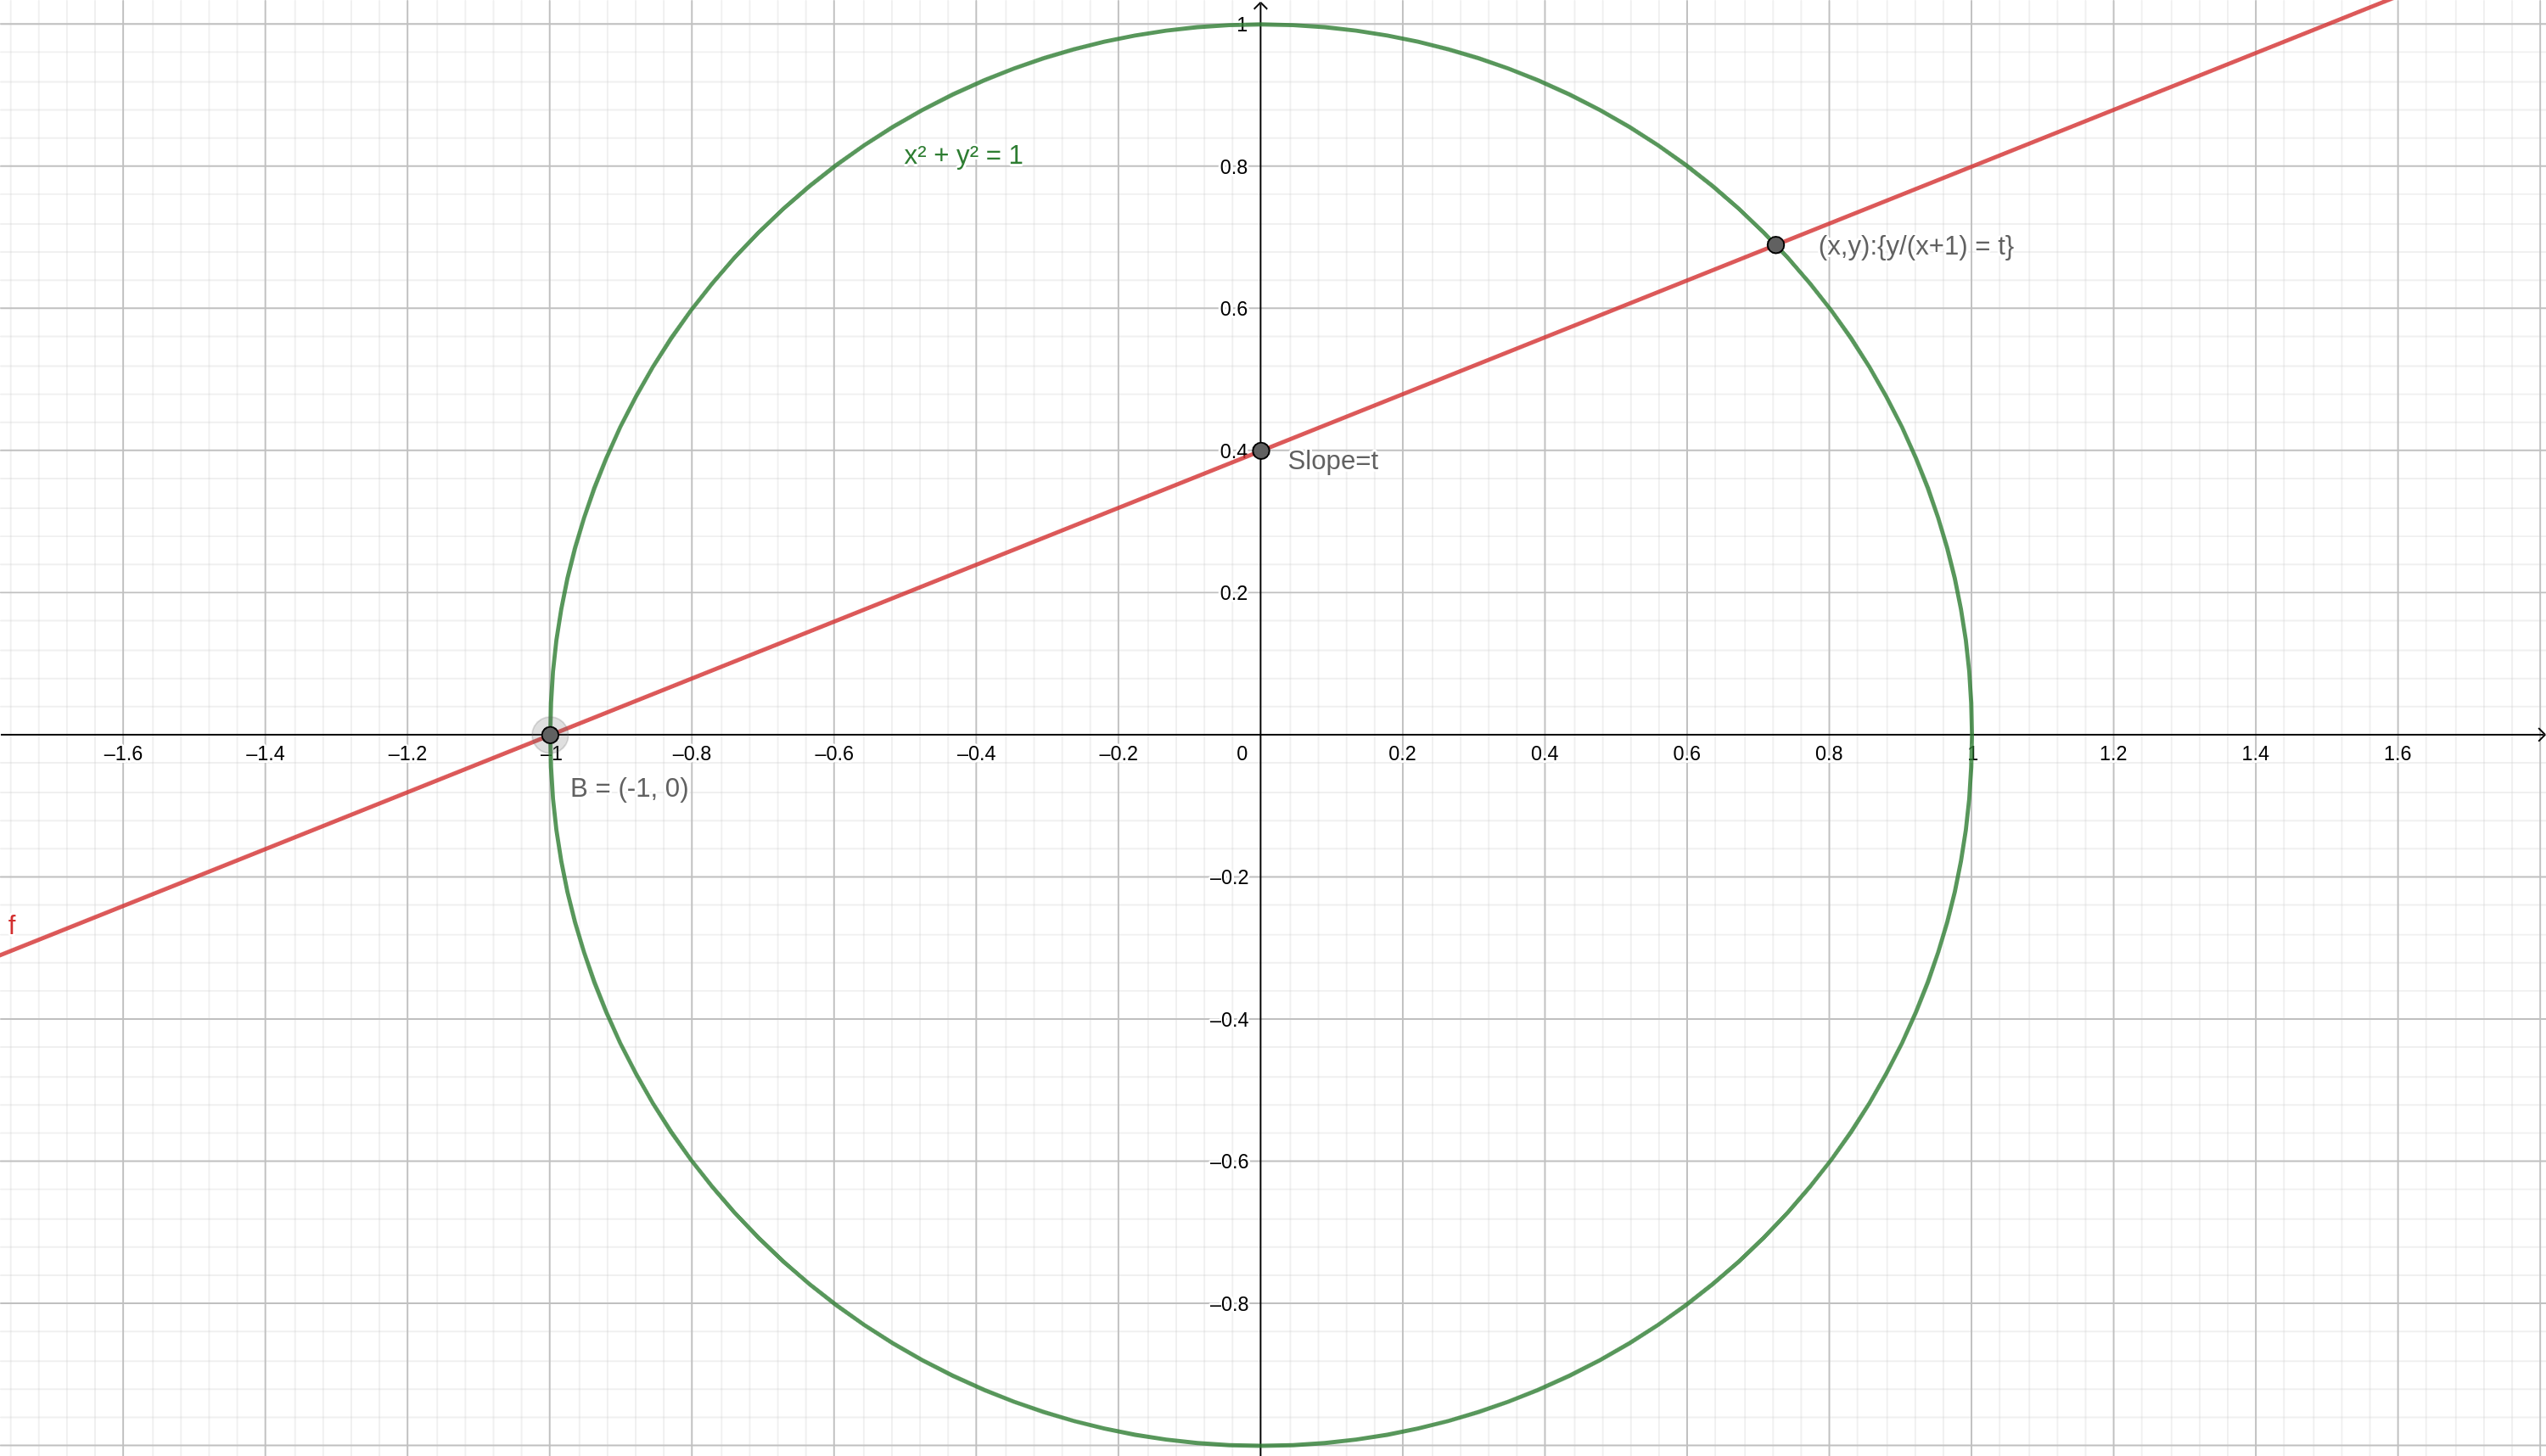
\includegraphics[width=0.9 \linewidth]{Pythagorean_circle.png}}
        \caption{Finding rational points with a line of rational slope}
        \label{fig:pyth_circle}
\end{figure}

Replacing $x = \frac{a}{c}, y = \frac{b}{c}$, we can see that finding integer solutions to $a^2 + b^2 = c^2$
is equivalent to finding rational solutions to $x^2 + y^2 = 1$. This is the equation of a circle of radius 1,
centered on the origin.

If we can find a way to find all rational points on the perimeter of the circle, then we will have found all
possible pythagrean triples, up to multiplication by a scalar (since if $a^2 + b^2 = c^2$, then
$(ka)^2 + (kb)^2 = (kc)^2$ for all $k \in \mathbb{Z}$). One way we can do that is to find one rational
point on the circle (say, $(0,-1)$, and draw lines through that point with a rational slope. We can show
that, since the slope of the line is rational, and the equation of the circle has integer coefficients, then
if one intersection point is rational (as it is by design), then the other point must also be rational.

Let's take an example to see how it happens. The line of slope $t$ through $(x,y) = (-1,0)$ is:
\[ y = tx +t\]

Clearly, $(-1,0)$ is on this line. Now, substituting this value of $y$ into the equation of the circle,
we get:
\[x^2 + (tx+t)^2 = (1+t^2)x^2 +2t^2x + t^2 -1 = 0 \]
And solving for $x$ we get $x = -1$ or $x = \frac{1-t^2}{1+t^2}$. Substituting this value of $x$ back into
our line, we get $y = \frac{2t}{1+t^2}$. We can easily verify that for any value of $t$ that this satisfies
the equation of the circle, as expected. And since $t$ is rational, $x$ and $y$ are guaranteed to be
rational too.

If we draw this line on the circle, we see that it has a $y$ intercept of $(x,y) = (0,t)$.

Is it possible, though, that we would somehow miss rational points in the circle by this method? 
In fact, a line between a rational point $(x,y)$ and $(-1,0)$ is $\frac{y}{x+1}$ and since $(x,y)$ is
a rational point, this is guaranteed to be rational too. So by enumerating all of the rational numbers
for line slopes, we are guaranteed to hit all of the rational numbers.

If we take the slope to be $t = \frac{m}{n}$ for $m,n \in \mathbb{Z}$ we can multiply across the
top and bottom by $n^2$ in the formulas for $x = \frac{1-t^2}{1+t^2}, y = \frac{2t}{1+t^2}$ to give
the Pythagorean triples $a = n^2-m^2, b = 2mn, c = n^2 + m^2$ for the familiar formula we found above.

Taking this approach with our problem, we substitute $x = \frac{a}{c}, y = \frac{b}{c}$ to get the equation:
\[ x^2 - xy + y^2 = 1 \]

\begin{figure}[htb]
        \center{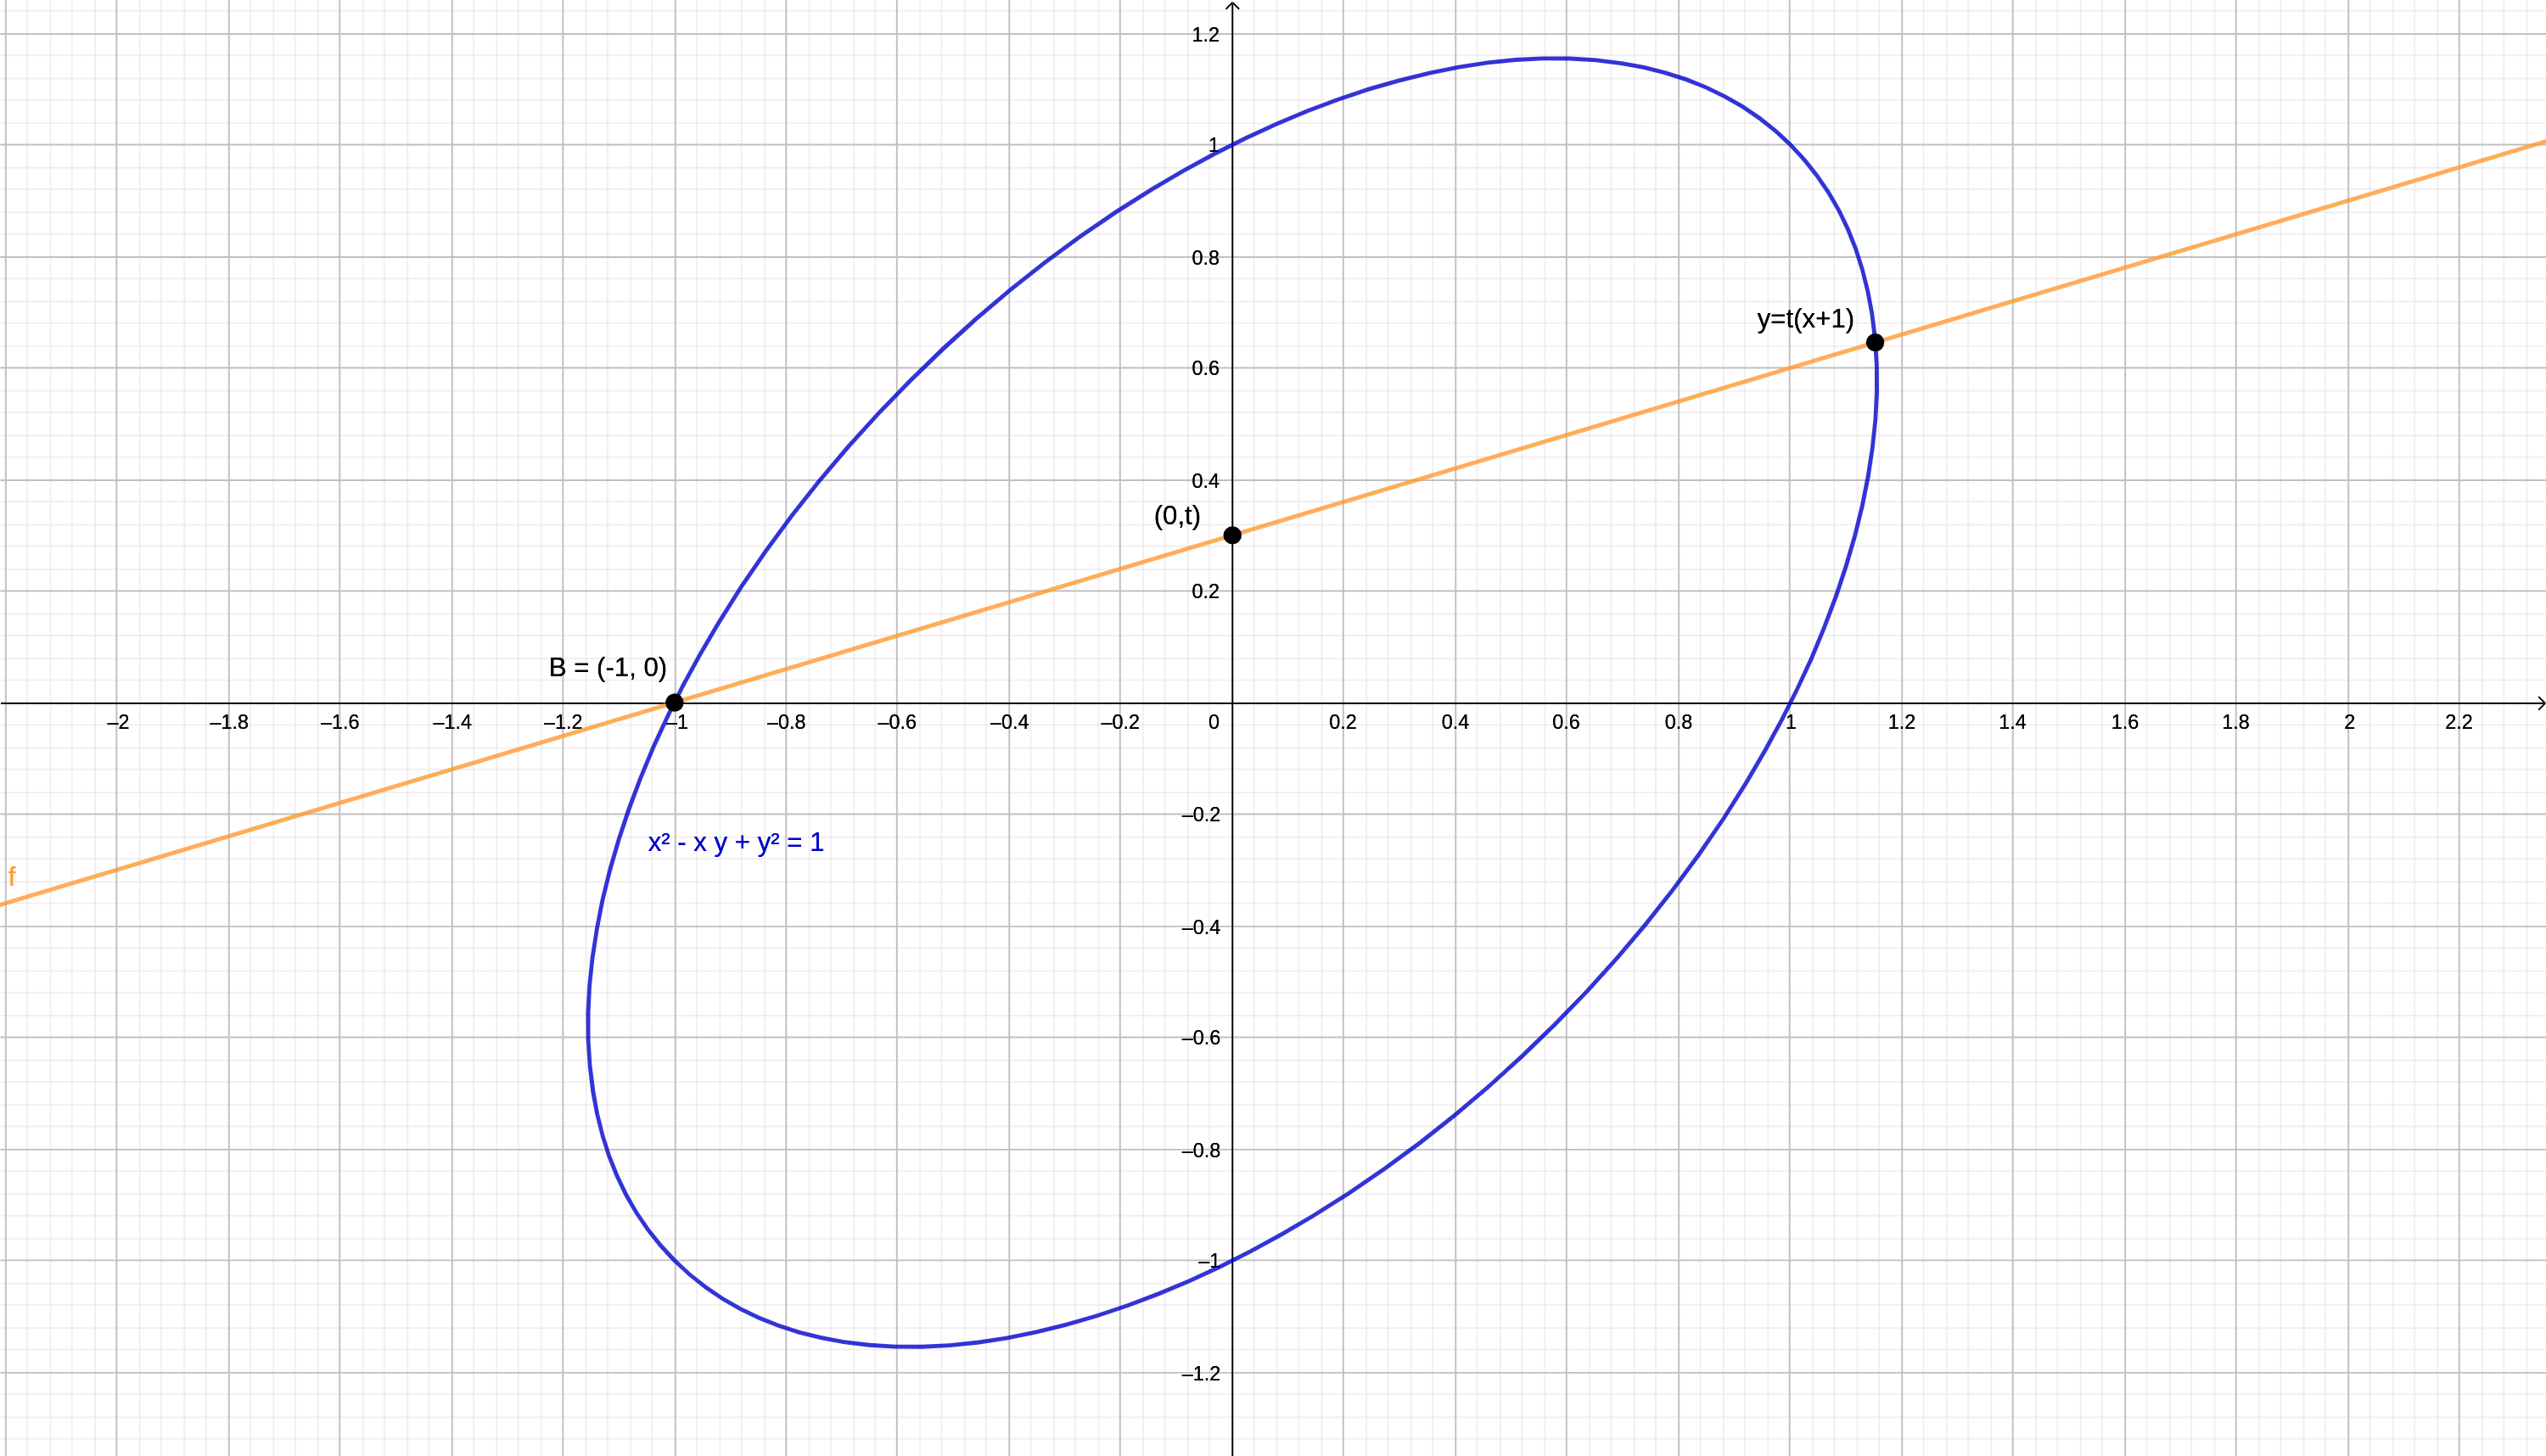
\includegraphics[width=0.9 \linewidth]{Eisenstein_ellipse.png}}
        \caption{Finding rational points with a line of rational slope}
        \label{fig:eisen_ellipse}
\end{figure}

This is an ellipse, centered on the origin, which goes through the points $(0,-1), (0,1), (-1,0), (1,0)$
on the X and Y axis. There are also a few other "nice" rational points on the curve at $(-1,-1), (1,1)$.

Now taking the same approach, given any rational number $t$, we can find the intersection points of our
ellipse and the line $y = t(x+1)$ (which again goes through $(-1,0)$):

\begin{equation*}
        \begin{split}
		x^2 - xy + y^2 & = x^2 - tx(x+1)+t^2(x+1)^2 \\
		&= (1-t+t^2)x^2 +(2t^2-t)x + t^2 \\
		&= 1 
	\end{split}
\end{equation*}

Now factoring to find the intersection points, we find, as expected, one of the points at $x=-1$, and
the other is a rational function of $t$:
\begin{equation*}
	\begin{split}
		(1-t+t^2)x^2 + (2t^2-t)x + (t^2-1) &= 0 \\
		(x + 1)((1-t+t^2)x + (t^2 - 1)) = 0
        \end{split}
\end{equation*}

So we have $x = -1$ or $x = \frac{1 - t^2}{1-t+t^2}$ for rational $t$.

Substituting the valie for $x$ back into the equation for the line:
\[ y = t(x+1) = \frac{2t - t^2}{1-t+t^2} \]

And replacing $t = \frac{m}{n}$ and multiplying through with $n^2$ above and below the line we get:
\[(x,y) = \left(\frac{n^2-m^2}{n^2-mn+m^2}, \frac{2nm - m^2}{n^2-mn+ m^2}\right) \]

And clearing a common denominator, we get an integer triple
$(a,b,c) = (n^2 - m^2, 2nm - m^2, m^2 - mn + n^2)$ as before.

A similar argument as before shows that this will find \textbf{all} rational points on the
ellipse, giving all integer solutions to the original problem (after dividing out any common factors
of $a, b, c$).


\end{document}
